% !Mode:: "TeX:UTF-8"
%%% Local Variables:
%%% mode: latex
%%% TeX-master: t
%%% End:

%面向对象的遥感影像的区间二型模糊聚类分割算法
\chapter{基于CGAN 影像分类的改进方法}
\label{cha:chap04}

\section{引言}
\label{sec:chap04-1}
在第~\ref{cha:chap03} 章中,我们将对抗训练的思想应用到FCN 分类模型中,提出了基于CGAN 影像分类方法。模型的对抗损失一定程度上增强了影像像素点间的连续性,提高了FCN 方法的影像分类效果。然而,因为遥感数据固有的不确定性,相比自然图像,遥感影像分类地物边界混淆、歧义性较严重。此外,模型中反卷积上采样操作将特征图恢复到原始影像尺寸,特征的损失也加剧了地物分类的边界模糊问题。因此,本章试图从增强影像分类结果边界信息和分割结果后处理两个角度改进基于CGAN 的遥感影像分类方法。本文作者于2017年研究过高分影像数据不确定性特征处理相关的内容,提出一种基于三角形模糊集值的区间二型模糊聚类方法(Triangular Fuzzy Set Valued Interval Type 2 Fuzzy Clustering Method, TFSV-IT2FCM) 方法\cite{jiang2018enhanced} 用于区分高分影像地物,且取得了较好的效果。影像聚类分割结果为许多同质性的分割单元,不同地物分类边界往往在分割单元间的边界线上。因此,本章将经TFSV-IT2FCM 聚类分割得到的影像分割单元图作为辅助信息,用于改进基于CGAN 影像分类方法。


\section{TFSV-IT2FCM 聚类分割}
\label{sec:chap04-2}

\subsection{方法原理}
\label{subsec:chap04-2-1}
由于遥感影像数据存在不确定性和混合边界问题,模糊C均值聚类(Fuzzy c-means clustering, FCM)方法被广泛应用到遥感影像解译中\cite{bezdek1984fcm}。随着高分影像数据的普及,遥感影像模糊聚类方法由基于像元的聚类方法发展为面向对象的模糊聚类方法。本文作者提出的TFSV-IT2FCM 方法就是面向对象的高分影像模糊聚类分割方法。TFSV-IT2FCM 算法首先定义三角形模糊集数据模型(Triangular Fuzzy Set Valued, TFSV)对高分影像的分割单元建模,能够表征影像分割单元内的像素点特征。然后定义一种新的区间值距离来度量两个TSFV 数的相似性。最后基于TFSV 数据模型和新的距离度量提出TFSV-ITFCM 模糊聚类方法。TFSV-ITFCM 聚类分割结果为许多同质性的聚类簇。各聚类簇的像素点差异性不大,且对簇内像素点变化具有一定容忍度。即某一簇内的所有像素点可视作同类地物。

\begin{figure}[!h]
    \centering
    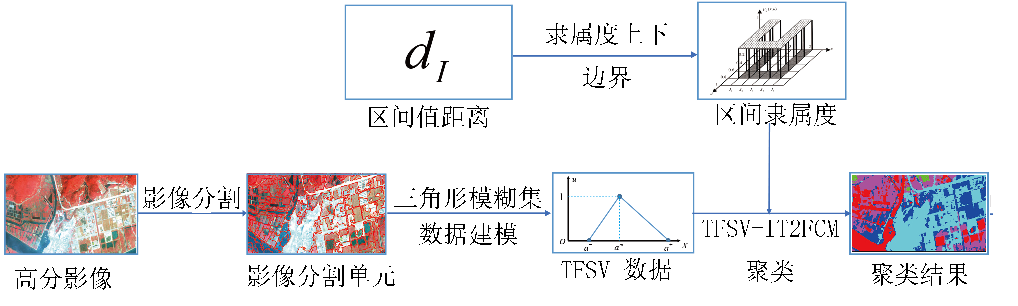
\includegraphics[width=0.9\textwidth]{figures/tfsvit2fcm}
    \caption{TFSV-IT2FCM 算法框架}
    \label{fig:tfsvit2fcm}
\end{figure}

TFSV-IT2FCM 方法的整体框架如图\ref{fig:tfsvit2fcm} 所示。首先对高分影像$\bm{I}$ ,使用SLIC 分割算法获得较小的影像分割单元 $\bm{SS}$,为:
\begin{equation}\label{eq:image_ss}
    \begin{split}
        \bm{SS} = \lbrace \bm{B_1}, \bm{B_2},\bm{\cdots}, \bm{B_n} \rbrace
    \end{split}
\end{equation}
其中$\bm{B_i}(1 \leq i \leq n)$ 表示第$i$ 个分割单元,$n$ 表示分割单元的总数。 $\bm{B_i}(i=1,2,\cdots, n)$ 是一个$j \times p$ 矩阵,其中$j$ 表示每个波段包含的像素数目,$p$ 表示图像通道数。对任一个影像单元$\bm{B_i}$ 均可以定义为一个TFSV 数据模型$\bm{\tilde{A_i}}$,影像分割单元的数据不确定性特征可由$\bm{\tilde{A_i}}$表达。即影像所有分割单元集合$\bm{SS} = \lbrace \bm{B_1}, \bm{B_2},\bm{\cdots}, \bm{B_n} \rbrace$ 可以被表示为:

\begin{equation}\label{eq:eq-2}
    \bm{SS} \to \lbrace \bm{\tilde{A_1}}, \bm{\tilde{A_2}},\bm{\cdots}, \bm{\tilde{A_n}} \rbrace
\end{equation}
其中$\bm{SS}$ 是一个$n \times p$ 矩阵,$\bm{\tilde{A_i}}$ 是$\bm{B_i}$ 对应的$p$ 维TFSV 数据,$n$ 表示分割单元的数目。$d_I$ 是定义TFSV 数据模型间的区间值距离,对于两个TFSV 数据$\tilde{A}$ 和$\tilde{B}$ 的区间值距离$d_I (\tilde{A}, \tilde{B})$ 为下式:
\begin{equation}\label{eq:interval}
    \begin{split}
        d _{I} (\tilde{A},\tilde{B}) = [\min \lbrace d_0 (\tilde{A},\tilde{B}),d_1(\tilde{A},\tilde{B}) \rbrace, \max \lbrace d_0(\tilde{A},\tilde{B}), d_1 (\tilde{A},\tilde{B}) \rbrace ]
    \end{split}
\end{equation}
式中$d_0 (\tilde{A},\tilde{B})$ 和$d_1 (\tilde{A},\tilde{B})$ 分别为$\tilde{A}$ 和$\tilde{B}$ 的$0-cut$ 和$ 1-cut$ 豪斯多夫距离\cite{zadeh1978fuzzy}。区间二型模糊聚类模型的隶属度上界$\overline{u}_{ij}$ 和下界$\underline{u}_{ij}$隶属度则由区间值距离$d _{I} $ 和模糊指数$m$ 求解,分别为:
\begin{equation}\label{eq:13}
    \begin{split}
        \overline{u}_{ij} = \max \Bigg \lbrace \frac{1}{\sum_{k=1}^K {(\frac{d_{ji}^0}{d_{ki}^0})}^{\frac{2}{m-1}}}, \frac{1}{\sum_{k=1}^K {(\frac{d_{ji}^1}{d_{ki}^1})}^{\frac{2}{m-1}}} \Bigg \rbrace
    \end{split}
\end{equation}
和
\begin{equation}\label{eq:14}
    \begin{split}
        \underline{u}_{ij} = \min \Bigg \lbrace \frac{1}{\sum_{k=1}^K {(\frac{d_{ji}^0}{d_{ki}^0})}^{\frac{2}{m-1}}}, \frac{1}{\sum_{k=1}^K {(\frac{d_{ji}^1}{d_{ki}^1})}^{\frac{2}{m-1}}} \Bigg \rbrace
    \end{split}
\end{equation}
其中$d_{ji}^0$ 和$d_{ji}^1$ 分别是输入样本$\tilde{X_i}$ 和聚类中心$\tilde{V_j}$ 的$0-cut$ 距离和$1-cut$ 距离度量,由区间值距离$d_{I} (\tilde{X_i}, \tilde{V_j})$ 计算得出。聚类迭代更新,求解区间二型的模糊划分矩阵$\bm{U} = [U_{ij}]_{n \times K}$
\begin{equation}\label{eq:21}
    U_{ij} = \frac{\underline{u}_{ij} + \overline{u}_{ij}}{2}
\end{equation}
其中 $U_{ij} = [\underline{u}_{ij}, \overline{u}_{ij}]$。然后,求出$\bm{\tilde{X}_i}$ 到聚类中心$\bm{\tilde{V}_k}$ 的最大隶属度$U_{ik}$ ,其中$k = 1, 2,\cdots, K$。最后根据最大隶属度原则,将$\bm{\tilde{X}_i}$ 划分到类别$\bm{\tilde{V}_k}$, 完成TFSV-IT2FCM 聚类分割过程。

TFSV-IT2FCM 聚类分割方法可以看作是对邻域内同质性像素点关系的建模,即邻域内具有相近像素值的像素点将被划分为同一个类别。此外,因模糊不确定度量的存在,同个聚类簇内的像素点可以在一定范围内波动。将TFSV-IT2FCM 聚类分割方法作用到高分影像,可以将各类别地物划分为不同的分类簇,而同一个簇内的像素点具有同质性,即更可能属于同一个地物类别,邻近簇之间的分界线也有很大机率为相邻的不同地物类别分类边界(也可能是同类地物的,当地物内部差异巨大时,同一地物会被模糊聚类为多个簇)。

\subsection{影像数据处理}
\label{subsec:chap04-2-2}
第\ref{cha:chap03} 章实验用到的Vaihingen 数据为$16$ 张尺寸约为$ 2563 \times 2049$ 的高分影像。为了得到影像整体的同质性分割单元信息图,这里直接使用TFSV-IT2FCM 聚类分割方法分别对这$16$ 张大尺寸影像聚类分割。因Vaihingen 数据共有地面、低矮植被、树木、建筑物、车辆、背景这六类地物,故TFSV-IT2FCM 聚类分割中聚类数可设置为六类。

图\ref{fig:tfsv_seg} 为TFSV-IT2FCM 方法提取Vaihingen影像同质性分割单元结果图。图\ref{fig:tfsv_seg}(a) 为Vaihingen 数据标号为$30$ 的影像,该影像尺寸为$1983\times2556$。使用TFSV-IT2FCM 聚类方法对影像进行分割,可以将影像依据分割单元的同质近似性,划分为许多个大小不一的簇,分割簇内的点输出标签相同,相邻簇间输出标签不同,图\ref{fig:tfsv_seg}(b) 即为影像聚类分割结果(聚类结果为一个波段二维矩阵,这里可视化三通道RGB 彩色图像),对分割单元信息图上依次经过图像梯度求解和二值化处理可以得到各个簇之间的边界信息,依据TFSV-IT2FCM 聚类分割结果提取到的影像边界信息如图\ref{fig:tfsv_seg}(c) 所示。 图\ref{fig:tfsv_seg}(d)为影响中间某区域的放大展示结果。

\begin{figure}[!h]
    \centering
    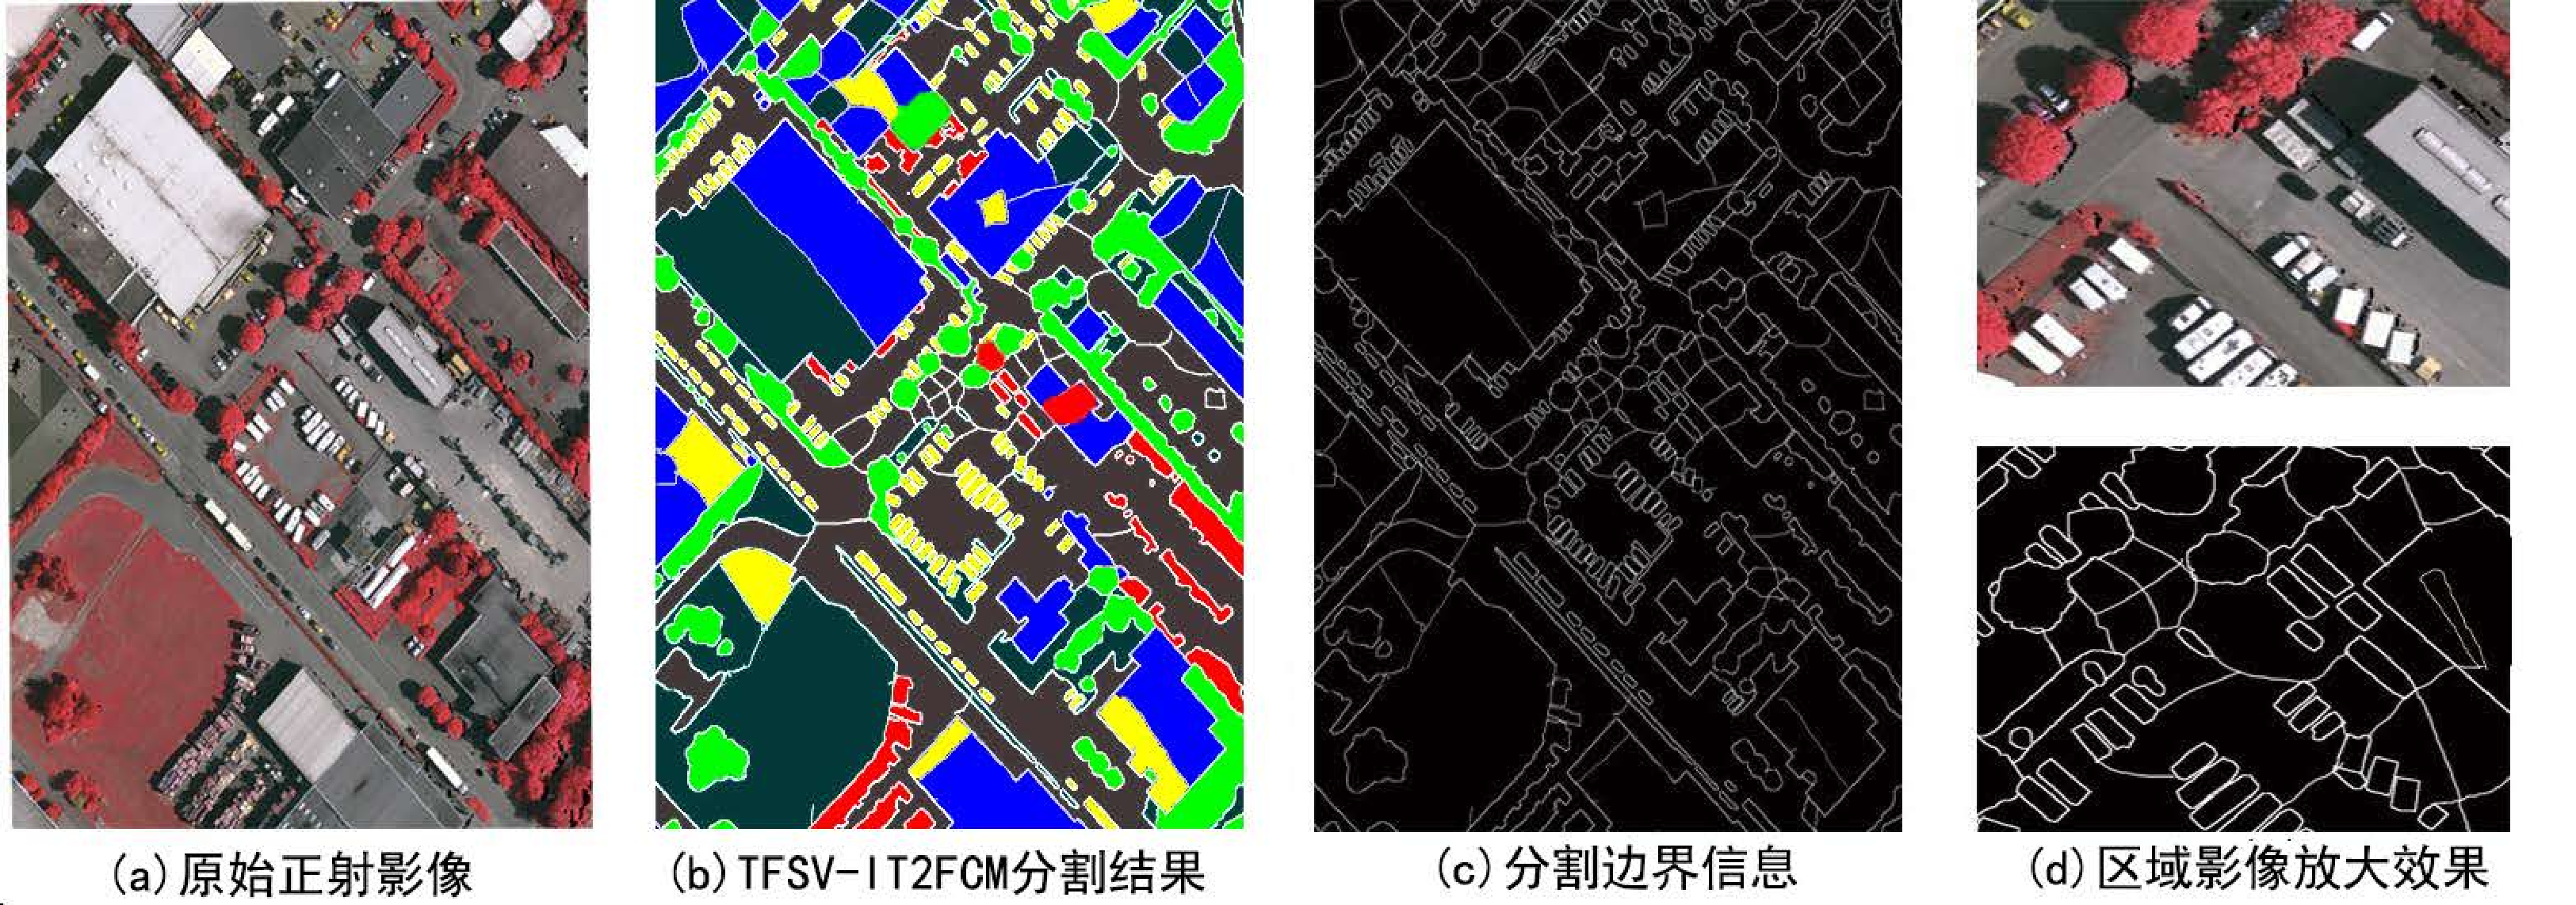
\includegraphics[width=1.0\textwidth]{figures/tfsv_seg}
    \caption{TFSV-IT2FCM 提取Vaihingen影像辅助特征信息}
    \label{fig:tfsv_seg}
\end{figure}

类似上面的处理方法,对Vaihingen 数据集内所有的$16$ 张影像均进行TFSV-IT2FCM 聚类分割操作,得到影像同质性分割单元图信息。数据聚类分割结果为二维的类别矩阵,这里将标签值采用最大最小归一化方法映射到$[0,1]$区间范围内。经过TFSV-IT2FCM聚类分割方法得到的影像边界辅助信息图与原始影像尺寸相同,且位置坐标一一对应。在第\ref{cha:chap03} 章随机滑动窗口裁切原始影像获取大小为$256\times 256$ 的训练样本时,也按照相同的滑窗裁切方式对同区域的影像辅助分割图进行裁切,得到训练样本边界辅助信息图。同理,待测试影像在按照规则网格裁切影像获取测试样本时也对测试影像的影像辅助分割图进行裁切。确保数据集所有样本同一区域的影像数据、类别标签图和经TFSV-IT2FCM 方法得到的影像辅助分割信息图三者一致对应。此外,利用TFSV-IT2FCM 方法获取影像辅助特征属于数据初始处理阶段,不会增加基于CGAN 的分类模型的迭代训练时间。


\section{融合边界特征的CGAN 影像分类方法}
\label{sec::chap04-4}

在上一小节中,我们使用TFSV-IT2FCM 聚类分割方法对高分影像数据做无监督聚类分割处理,使用TFSV 模型对影像数据不确定性建模,再对影像分割单元的TFSV 数据模型进行聚类。得到高分影像的同质性分割单元信息图。%聚类过程将影像划分为多个大小不一的分类簇。同一个分割单元簇内像素具有较强的类别一致性,簇之间的分割边界则有可能为异类地物的分割边界。对模型中所有的训练样本和测试样本均可获得由TFSV-IT2FCM 方法聚类分割得到的辅助边界特征信息图。


在基于CGAN 的影像分类方法中,生成网络的池化操作使得影像空间分辨率减小,影像像素点的位置信息不可避免的存在损失。此外,分割模型使用反卷积上采样操作扩大特征图的尺寸,像素点低阶位置信息丢失的更加严重。将影像低阶边界位置特征信息传到高层特征图中,一定程度上即可弥补因池化操作和上采样过程中像素点损失的位置信息。基于上一节得到的影像分割单元边界信息图,对分割模型中各级上采样输出的特征图融合相同尺度的边界掩膜特征信息,提升高阶语义特征的边界位置信息,对基于CGAN 的影像分类方法进行改进,提出融合边界掩膜特征的CGAN 影像分类方法。

\begin{figure}[!h]
    \centering
    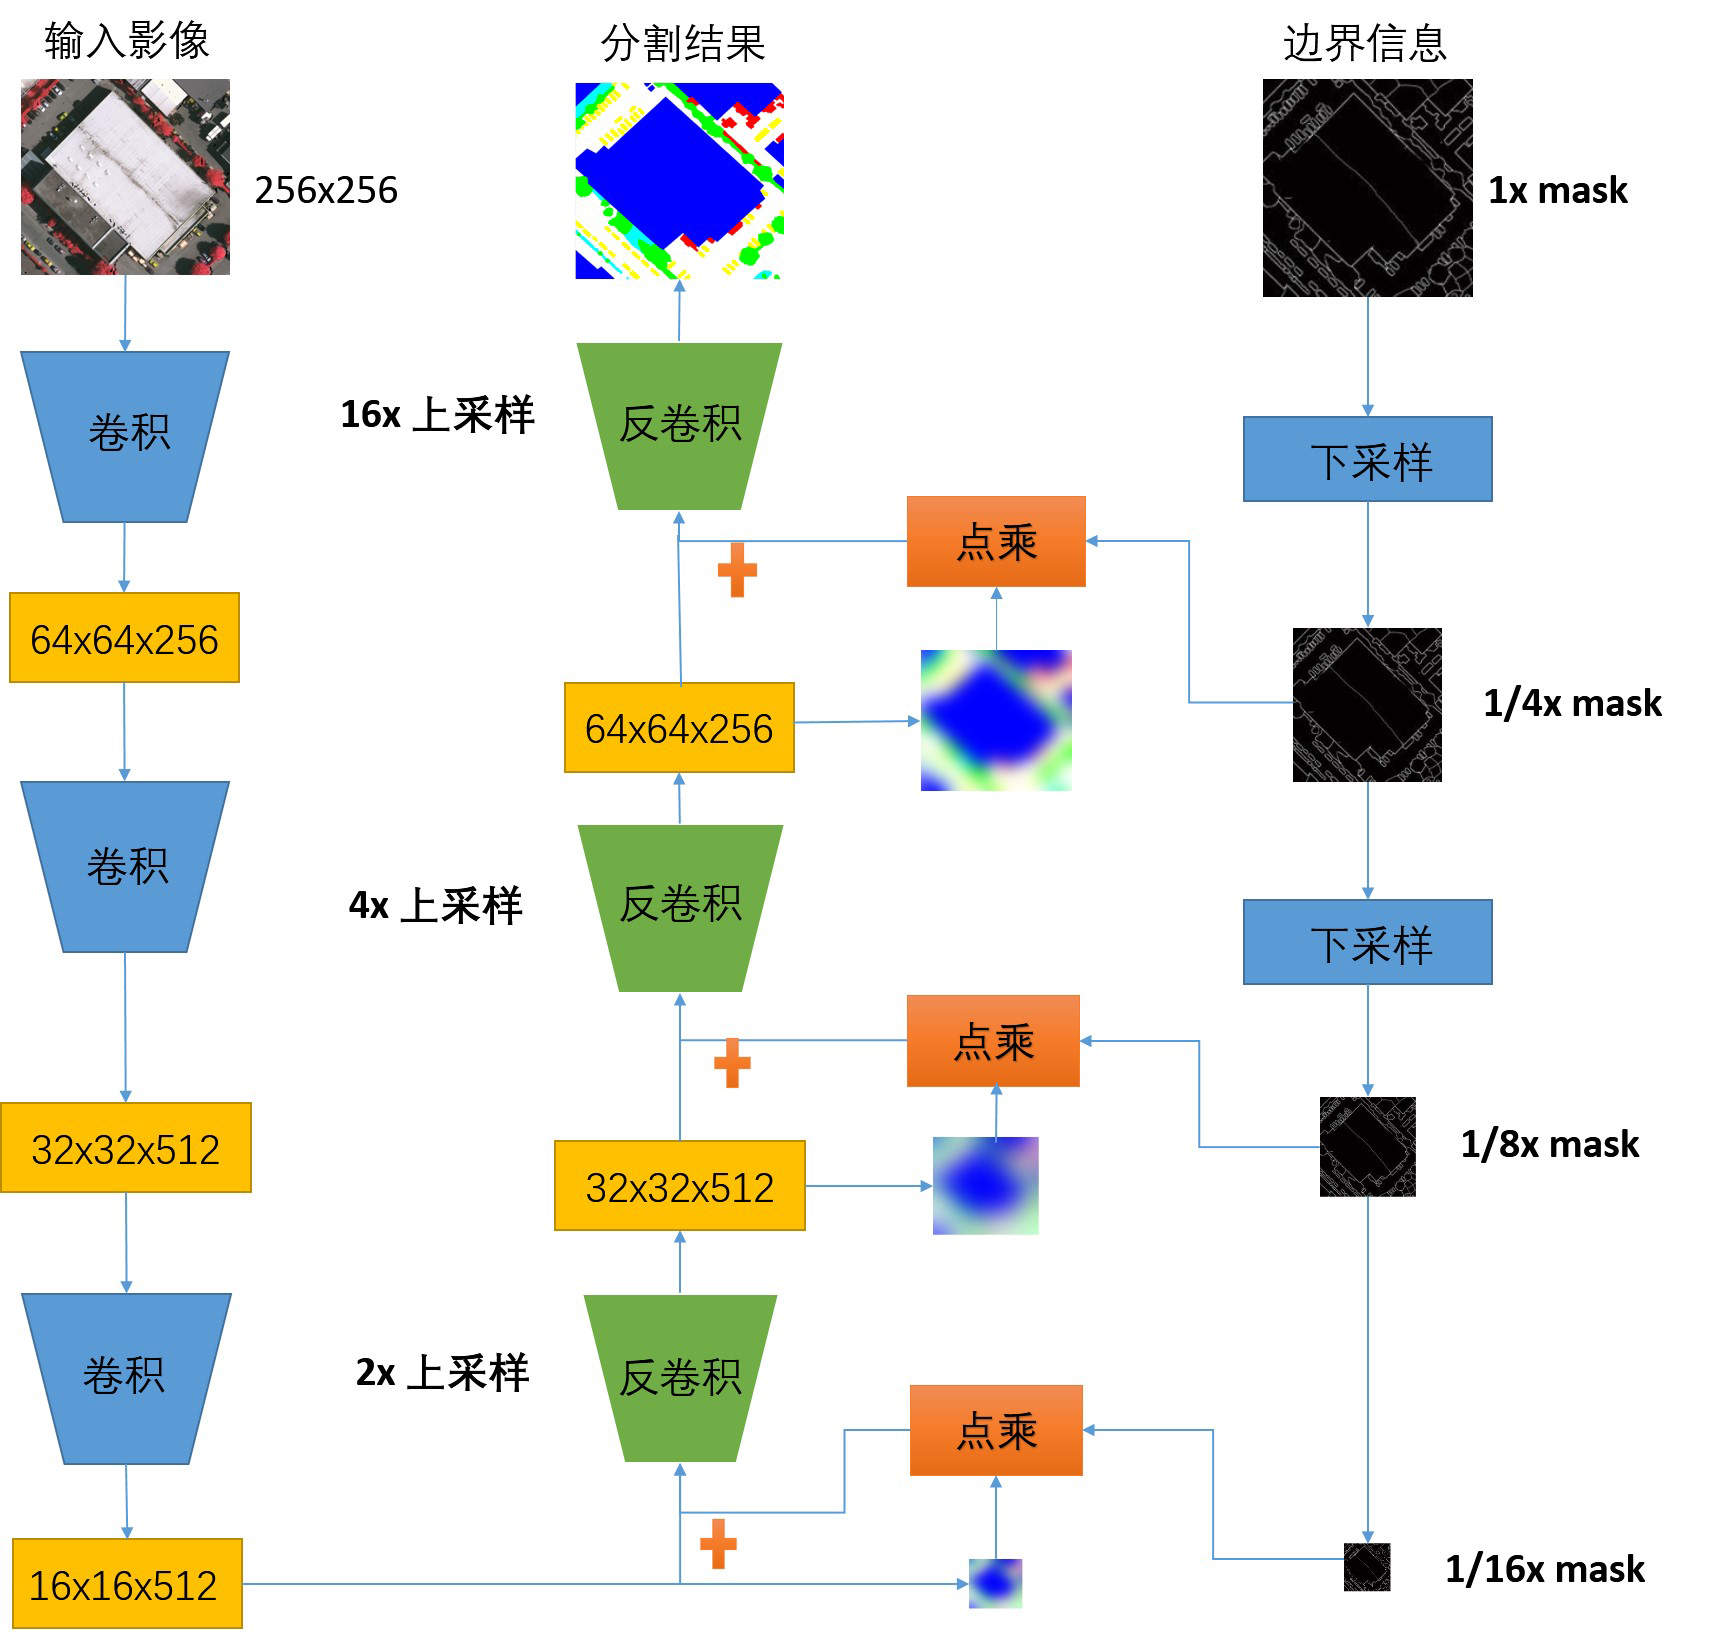
\includegraphics[width=1.0\textwidth]{figures/mask_gan}
    \caption{融合边界掩膜特征的分割模型}\label{fig:mask_gan}
\end{figure}

图\ref{fig:mask_gan} 所示为融合边界掩膜特征的CGAN 影像分类方法的生成器分割模型部分示意图。假设由TFSV-IT2FCM 聚类分割方法得到影像分割单元图为$S$,根据图像梯度求解$S$ 的边界信息,如式\ref{eq:n4-1} 所示,$S$ 上任一点$(x,y)$ 的梯度值可以求解得到,S 的梯度图表示为$S_g$。
\begin{equation}\label{eq:n4-1}
    \begin{split}
        |grad(S(x,y))| = [(\frac{\partial S}{\partial x})^2 + (\frac{\partial S}{\partial y})^2]^{\frac{1}{2}}
    \end{split}
\end{equation}
对梯度图$S_g$ 上的梯度进行二值化处理,如式\ref{eq:n4-2}即可得到影像边界掩膜信息$S_e$。
\begin{equation}\label{eq:n4-2}
    S_e(x,y) =
    \begin{cases}
        1, & |grad(S(x,y))| > 0 \\
        0, & |grad(S(x,y))| = 0
    \end{cases}
\end{equation}
边界掩膜$S_e$ 为单波段二值灰度灰度图,其图像初始尺寸与输入样本尺寸相同,为$256\times 256$。为了将掩膜融合到各级反卷积的特征输出图中,使用最大池化方法对掩膜图$S_e$ 按倍数进行下采样处理,分别得到$\frac{1}{4}$、$\frac{1}{8}$ 和$\frac{1}{16}$ 倍原始尺寸大小的边界掩膜特征图。借鉴ResNet\cite{he2016deep} 模型中“残差学习”组合特征的思想,我们对模型中各个层级的反卷积特征图融合对应尺度大小的边界特征信息。假设某一尺度反卷积层原始输入特征图为$X_f$,该层同尺度的边界掩膜为$S_e^m$,则添加掩膜融合后新的特征图$X_f^\star$ 可以表示为下式
\begin{equation}\label{eq:n4-3}
    X_f^\star = X_f + H(X_f, S_e^m)
\end{equation}
式中$ H(X_f, S_e^m)$ 为矩阵哈达玛积\cite{horn1990hadamard}(Hadamard product),也叫矩阵点乘。对于两个矩阵$A,B \in \mathbb{R}^{m\times n}$,且$A=\{a_{ij}\}$,$B=\{b_{ij}\}$,则$A$ 和$B$ 的哈达玛积为式\ref{eq:n4-4} 所示。
\begin{equation}\label{eq:n4-4}
    H(A,B) =
    \left[
        \begin{matrix}
            a_{11}b_{11} & a_{12}b_{12} & a_{13}b_{13} & \cdots & a_{1n}b_{1n} \\
            a_{21}b_{21} & a_{22}b_{22} & a_{23}b_{23} & \cdots & a_{2n}b_{2n} \\
            \vdots       & \vdots       & \vdots       & \ddots & \vdots       \\
            a_{m1}b_{m1} & a_{m2}b_{m2} & a_{m3}b_{m3} & \cdots & a_{mn}b_{mn} \\
        \end{matrix}
        \right]
\end{equation}
可以求出掩膜$S_e^m$ 和特征图为$X_f$ 矩阵对应位置元素的哈达玛积结果。使用融合边界掩膜的特征图$X_f^\star$ 替代$X_f$,参与网络模型迭代训练。对于各层反卷积的特征图均采取上述融合边界掩膜的方式,即将影像像素位置、边界等低层特征组合到反卷积阶段的高层语义特征中,提升模型对影像地物边界的识别能力。


% 第\ref{cha:chap03}章中基于CGAN 的影像分类方法使用正射影像和DSM 数据组成的四波段融合数据作为模型输入,能够得到最好的影像分类结果。这里,将聚类分割的辅助特征信息图作为影像新波段数据,融合到CGAN 模型样本中。


\section{基于辅助信息后处理的影像分类方法}
\label{sec::chap04-4}
上文中我们提出融合边界掩膜特征的CGAN 影像分类方法,将边界掩膜特征信息融合到高阶语义特征中,改善了影像像素点下采样过程中丢失位置、边界等低阶特征的问题。然而,基于CGAN 影像影像分类方法中分割模型最后一层输出为影像各像素点所属类别的概率分布。对各像素点分类预测只考虑了各像素点自身的概率分布,没有考虑到该像素点邻域内像素点间的关系,这样做的后果容易导致分类结果中出现很多细碎的错分区域。特别是高分影像中复杂特征的地物,同类别地物区域内的分割结果很容易出现细碎的错分区域。

影像中像素点通常满足局部相似性原则,即相邻像素之间往往更可能具有相同的类别标签,一定空间范围内相似颜色的像素点更可能具有相同的类别标签。基于上一节由TFSV-IT2FCM 聚类分割方法预处理得到的影像同质性分割单元图,我们对基于CGAN 影像分类模型中生成模型输出层结果做后处理操作,当前像素点分类标签不仅依赖于当前像素点预测类别的概率,还受当前像素点所处的影像分割单元中其他像素点的影响。


% 借鉴FCN 模型中跳跃连接弥补特征损失的思想,我们将上一节通过TFSV-IT2FCM 聚类方法得到的辅助分割信息图特征应用到分割模型输出层中,分类预测时考虑单个像素分类概率值和辅助分割信息图中同一分割单元内其他像素点的相互关系,优化分类图像中粗糙和不确定的像素的预测标签。这样既可减少同类地物中细碎的错分问题,同时又可以得到更精细、准确的地物分割边界。


设影像$X$ 由N个像素点组成,即有$X = \{X_1,X_2,\cdots,X_3\}$,共有$L$ 个类别地物的影像类别标签值为$L = \{l_1,l_2, \cdots, l_L \}$。对每个像素点$X_i$,基于CGAN 影像分类方法分割模型输出是经过Softmax 归一化的$L$ 维向量,如下式
\begin{equation}\label{eq:n4-4-1}
    P(X_i) = [P(X_i=l_1),P(X_i=l_2),\cdots,P(X_i=l_L)]
\end{equation}
其中$P(X_i=l_c)$ 表示像素点$X_i$ 被分为第$l_c(c=1,2,\cdots,L)$ 类地物的概率。模型类别决策时对式\ref{eq:n4-4-1} 使用argmax 函数做概率最大化划分类别维度即可。


本节研究内容就是优化这里的类别决策方式。假设预处理得到的同质性分割单元图为$S$,$S$ 为多个影像分割单元的集合,设某个分割单元内像素点集合为$X_S$,其包含$S$ 个像素点。对影像分割单元$X_S$内所有像素点统计各类别维度是当前像素点概率最大的类别标签的像素点个数,即有:
\begin{equation}\label{eq:n4-5}
    C = \{C^S_{l_1},C^S_{l_2}, \cdots, C^S_{l_L}\}
\end{equation}
且满足约束条件
\begin{equation}\label{eq:n4-6}
    S  = \sum _{i = 1}^L C^S_{l_i}
\end{equation}
式\ref{eq:n4-5} 中$C^S_{l_i}$ 表示当前分割单元$X_S$中满足分割模型预测像素点类别为$l_i$ 时概率最大的像素点的个数,总的像素点个数之和为$S$,即有式\ref{eq:n4-6}。对式\ref{eq:n4-5} 中每一项除以$S$,求出分割单元$X_S$中每一个类别标签为最大概率时的像素点个数占当前分割单元$X_S$总像点个数的比值,即
\begin{equation}\label{eq:n4-7}
    P_s(l_i) = \frac{C^S_{l_i}}{S},i=1,2,\cdots,L
\end{equation}

利用式\ref{eq:n4-7} 中分割单元的占比关系,对式\ref{eq:n4-4} 中像素点类别预测的概率值进行更新,更新方法如式\ref{eq:n4-8}所示:
\begin{equation}\label{eq:n4-8}
    P^{\star}(X_i=l_c) =  P(X_i=l_c) + \lambda \times \exp{(P_s(l_c)-1)}
\end{equation}
式中 $\lambda$ 为权衡因子,取值范围为$[0,1]$,是一个超参数,在后面实验中取$\lambda=0.8$ 能得到最好的实验效果。$P_s(l_c)$ 为$[0,1]$ 内的一个比值,比值$P_s(l_c)$ 越大,表明该影像分割单元区域内预测为该类别的像素点占据多数,式\ref{eq:n4-8} 对该类别标签的预测概率有正向加权激励作用,符合影像邻近相似像素更可能为同类标签的准则。


\begin{figure}[htbp]
    \centering
    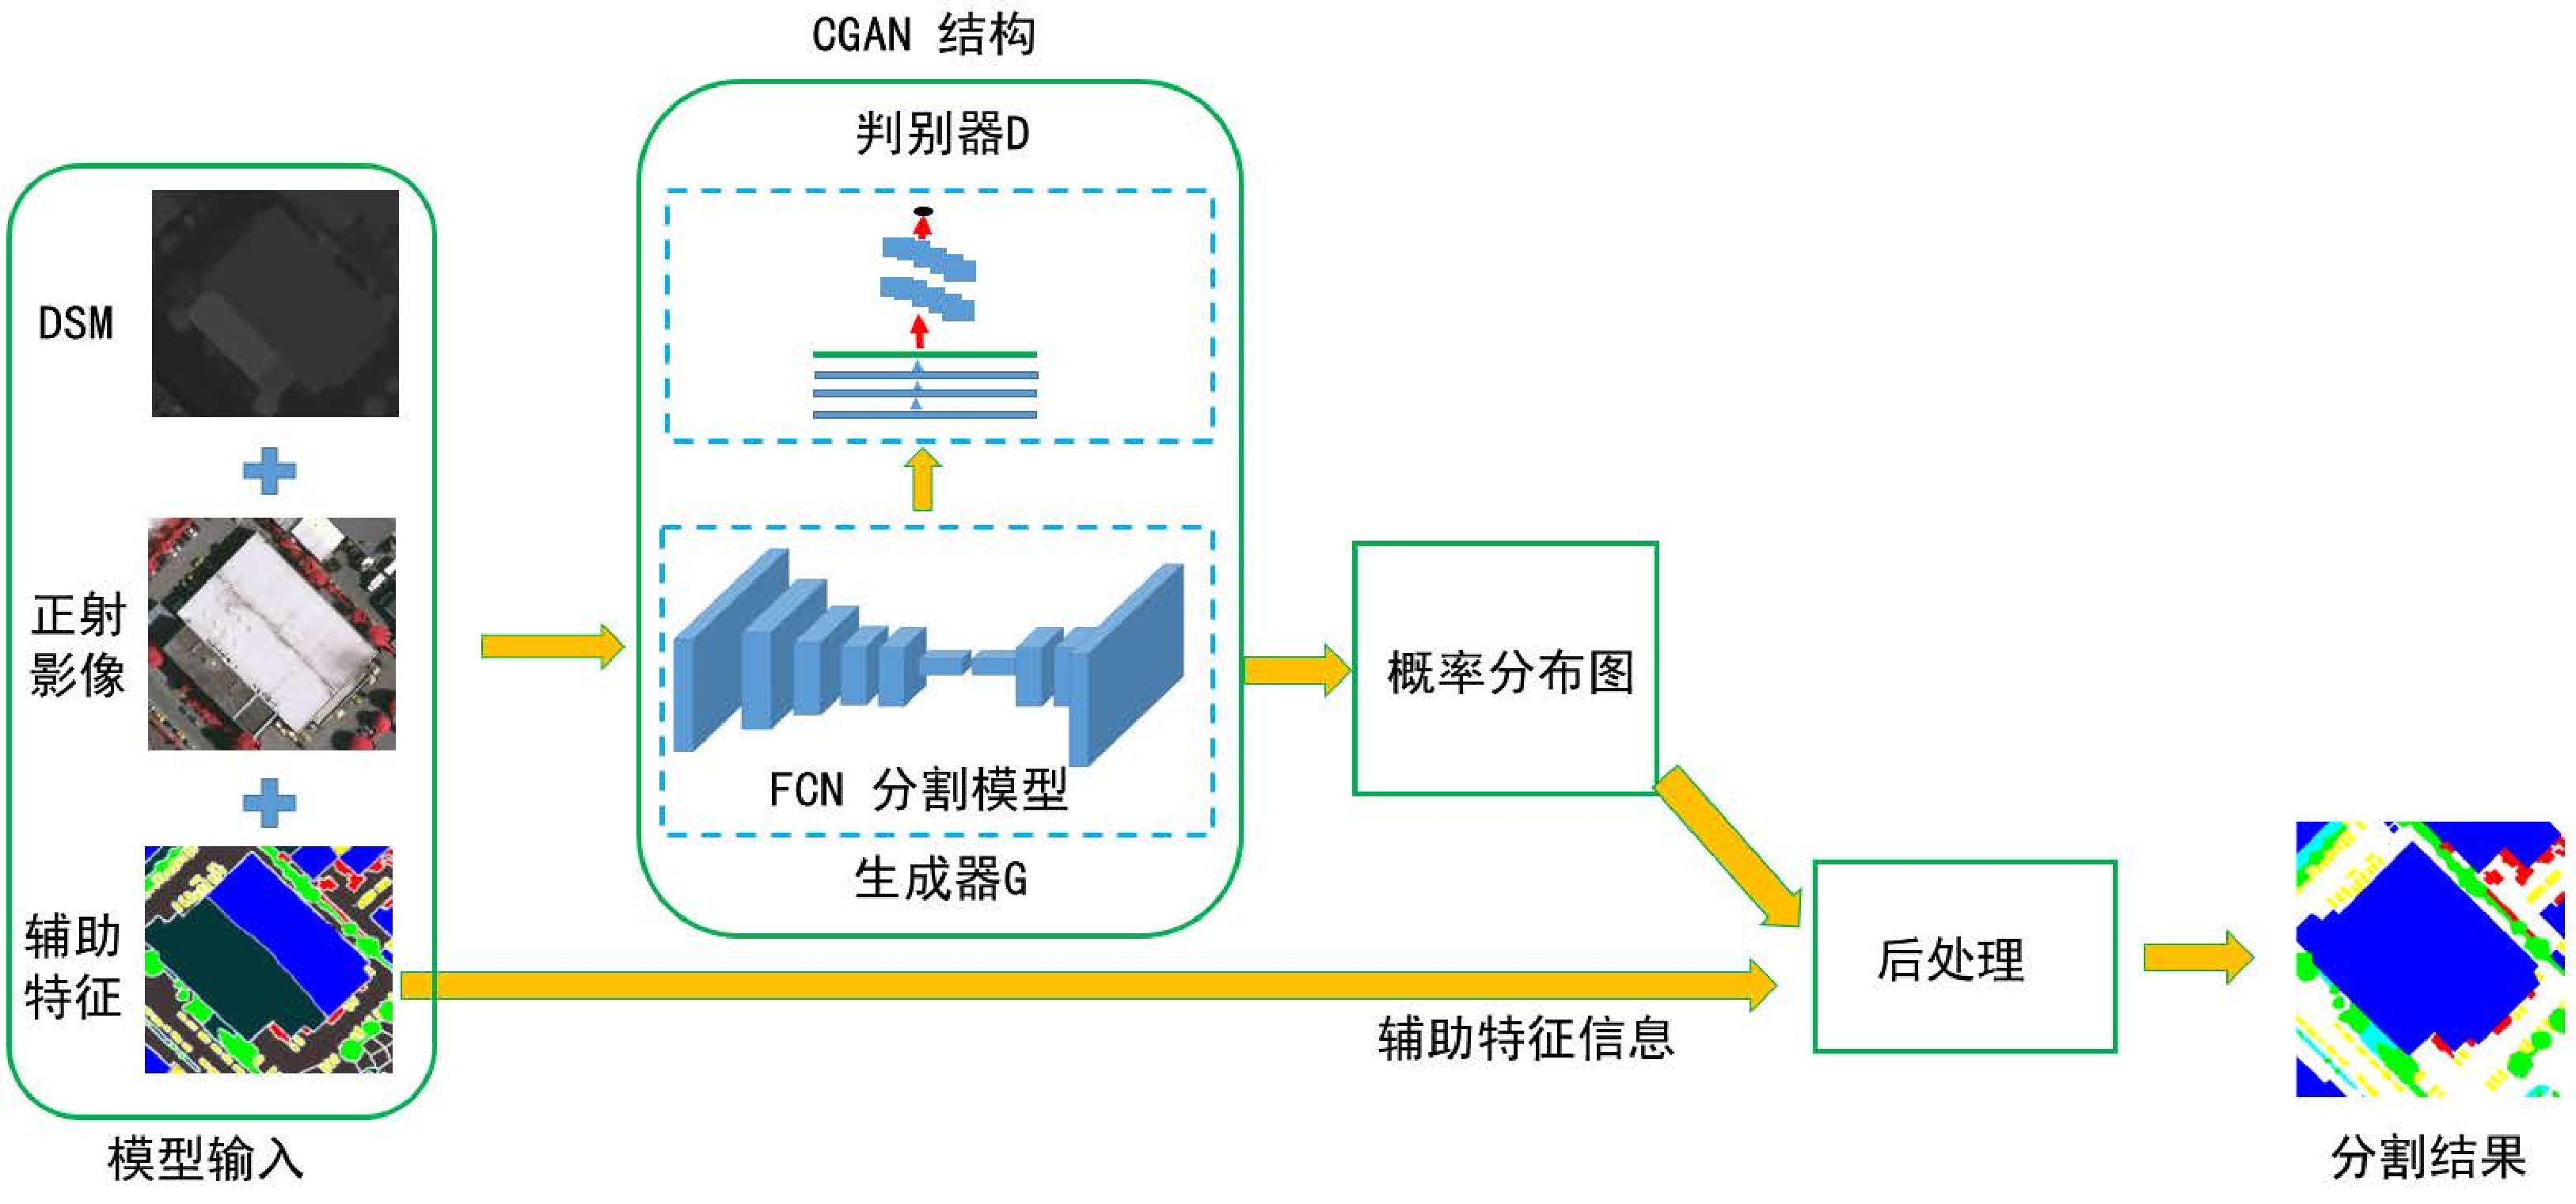
\includegraphics[width=1.0\textwidth]{figures/cgan_post}
    \caption{基于辅助信息后处理的CGAN 影像分类流程图 }\label{fig:cgan_post}
\end{figure}

在模型训练迭代时,使用式\ref{eq:n4-8} 中概率分布结果代替分割模型预测输出概率,即式\ref{eq:4-5} 中基于CGAN 影像分类方法分割网络的多分类交叉熵损失更新为下式:
\begin{equation}
    \label{eq:n4-9}
    l_{mce} (\hat{y}, y) = -\sum_{i=1}^{H\times W}\sum_{c=1}^{C}y_{ic}\log(\hat{y}_{ic} + \lambda \times \exp(P_s(l_c)-1))
\end{equation}
将式\ref{eq:n4-9} 中多分类交叉损失更新到基于CGAN 分类模型的目标函数(式\ref{eq:4-7})中,进而对网络模型进行权值更新、迭代训练。基于辅助信息后处理的CGAN 影像分类方法流程如图\ref{fig:cgan_post} 所示,正射影像和DSM 数据作为模型输入,同质性分割单元图作为辅助信息更新生成模型输出层的概率分布图。
% \begin{equation}
%     \label{eq:4-5}
%     l_{mce} (\hat{y}, y) = -\sum_{i=1}^{H\times W}\sum_{c=1}^{C}y_{ic}\log()\hat{y}_{ic} + \lambda \times \exp^{(P_s(l_c)-1)}
%   \end{equation}


\section{实验结果与分析}
\label{sec::chap04-5}

基于CGAN 的影像分类模型中网络池化操作和反卷积上采样丢失了影像低阶的位置、边界信息,文中借助TFSV-IT2FCM 影像聚类分割方法获取影像的分割单元边界信息,然后将边界信息下采样到不同尺寸,以特征掩膜的方式融合到反卷积输入特征图中,增加高阶语义特征中的低阶边界特征。为了验证文中提出的融合边界掩膜特征的CGAN 影像分类方法的正确性。我们在Vaihingen 数据集上进行实验。实验环境和参数条件等配置跟第\ref{cha:chap03} 章的实验配置相同,分类效果的评价指标为OA 和mIoU。分类的量化评估结果如表\ref{tab:bianjie_cgan} 所示,可以发现整体的分类精度OA 和mIoU 相比没有融合边界特征的CGAN影像分类方法均有一定程度的提升,融合边界特征的CGAN 分类方法OA 提升了$3.34\%$,为$83.49\%$。mIoU 也从$61.83\%$ 提高到$63.52\%$。从地面、低矮植被、树木、建筑物、车辆这五类地物正确识别的精度来看,“车辆” 的分类精度提升幅度最大,为$4.75\%$。研究发现,相比其他类型地物,“车辆”在影像中的占比和像素区域大小均较小,融合边界特征后一定程度能够还原出影像上“车辆”这类地物的区域边界范围,因此,融合边界特征信息对影像小区域同类地物的识别改善效果最明显。

\begin{table}[!h]
    \centering
    \caption{融合边界特征对影像分类的影响}\label{tab:bianjie_cgan}
    \begin{tabular}{p{4cm}ccccccc}
        \toprule
        方法            & 地面      & 低矮植被  & 树木      & 建筑物    & 车辆      & OA        & mIoU      \\
        \midrule
        CGAN            & $83.78\%$ & $74.47\%$ & $82.40\%$ & $87.64\%$ & $78.83\%$ & $80.15\%$ & $61.83\%$ \\
        CGAN + 融合特征 & $82.54\%$ & $77.59\%$ & $83.21\%$ & $84.48\%$ & $83.58\%$ & $83.49\%$ & $63.52\%$ \\
        \bottomrule
    \end{tabular}
\end{table}

\begin{figure}[!h]
    \centering
    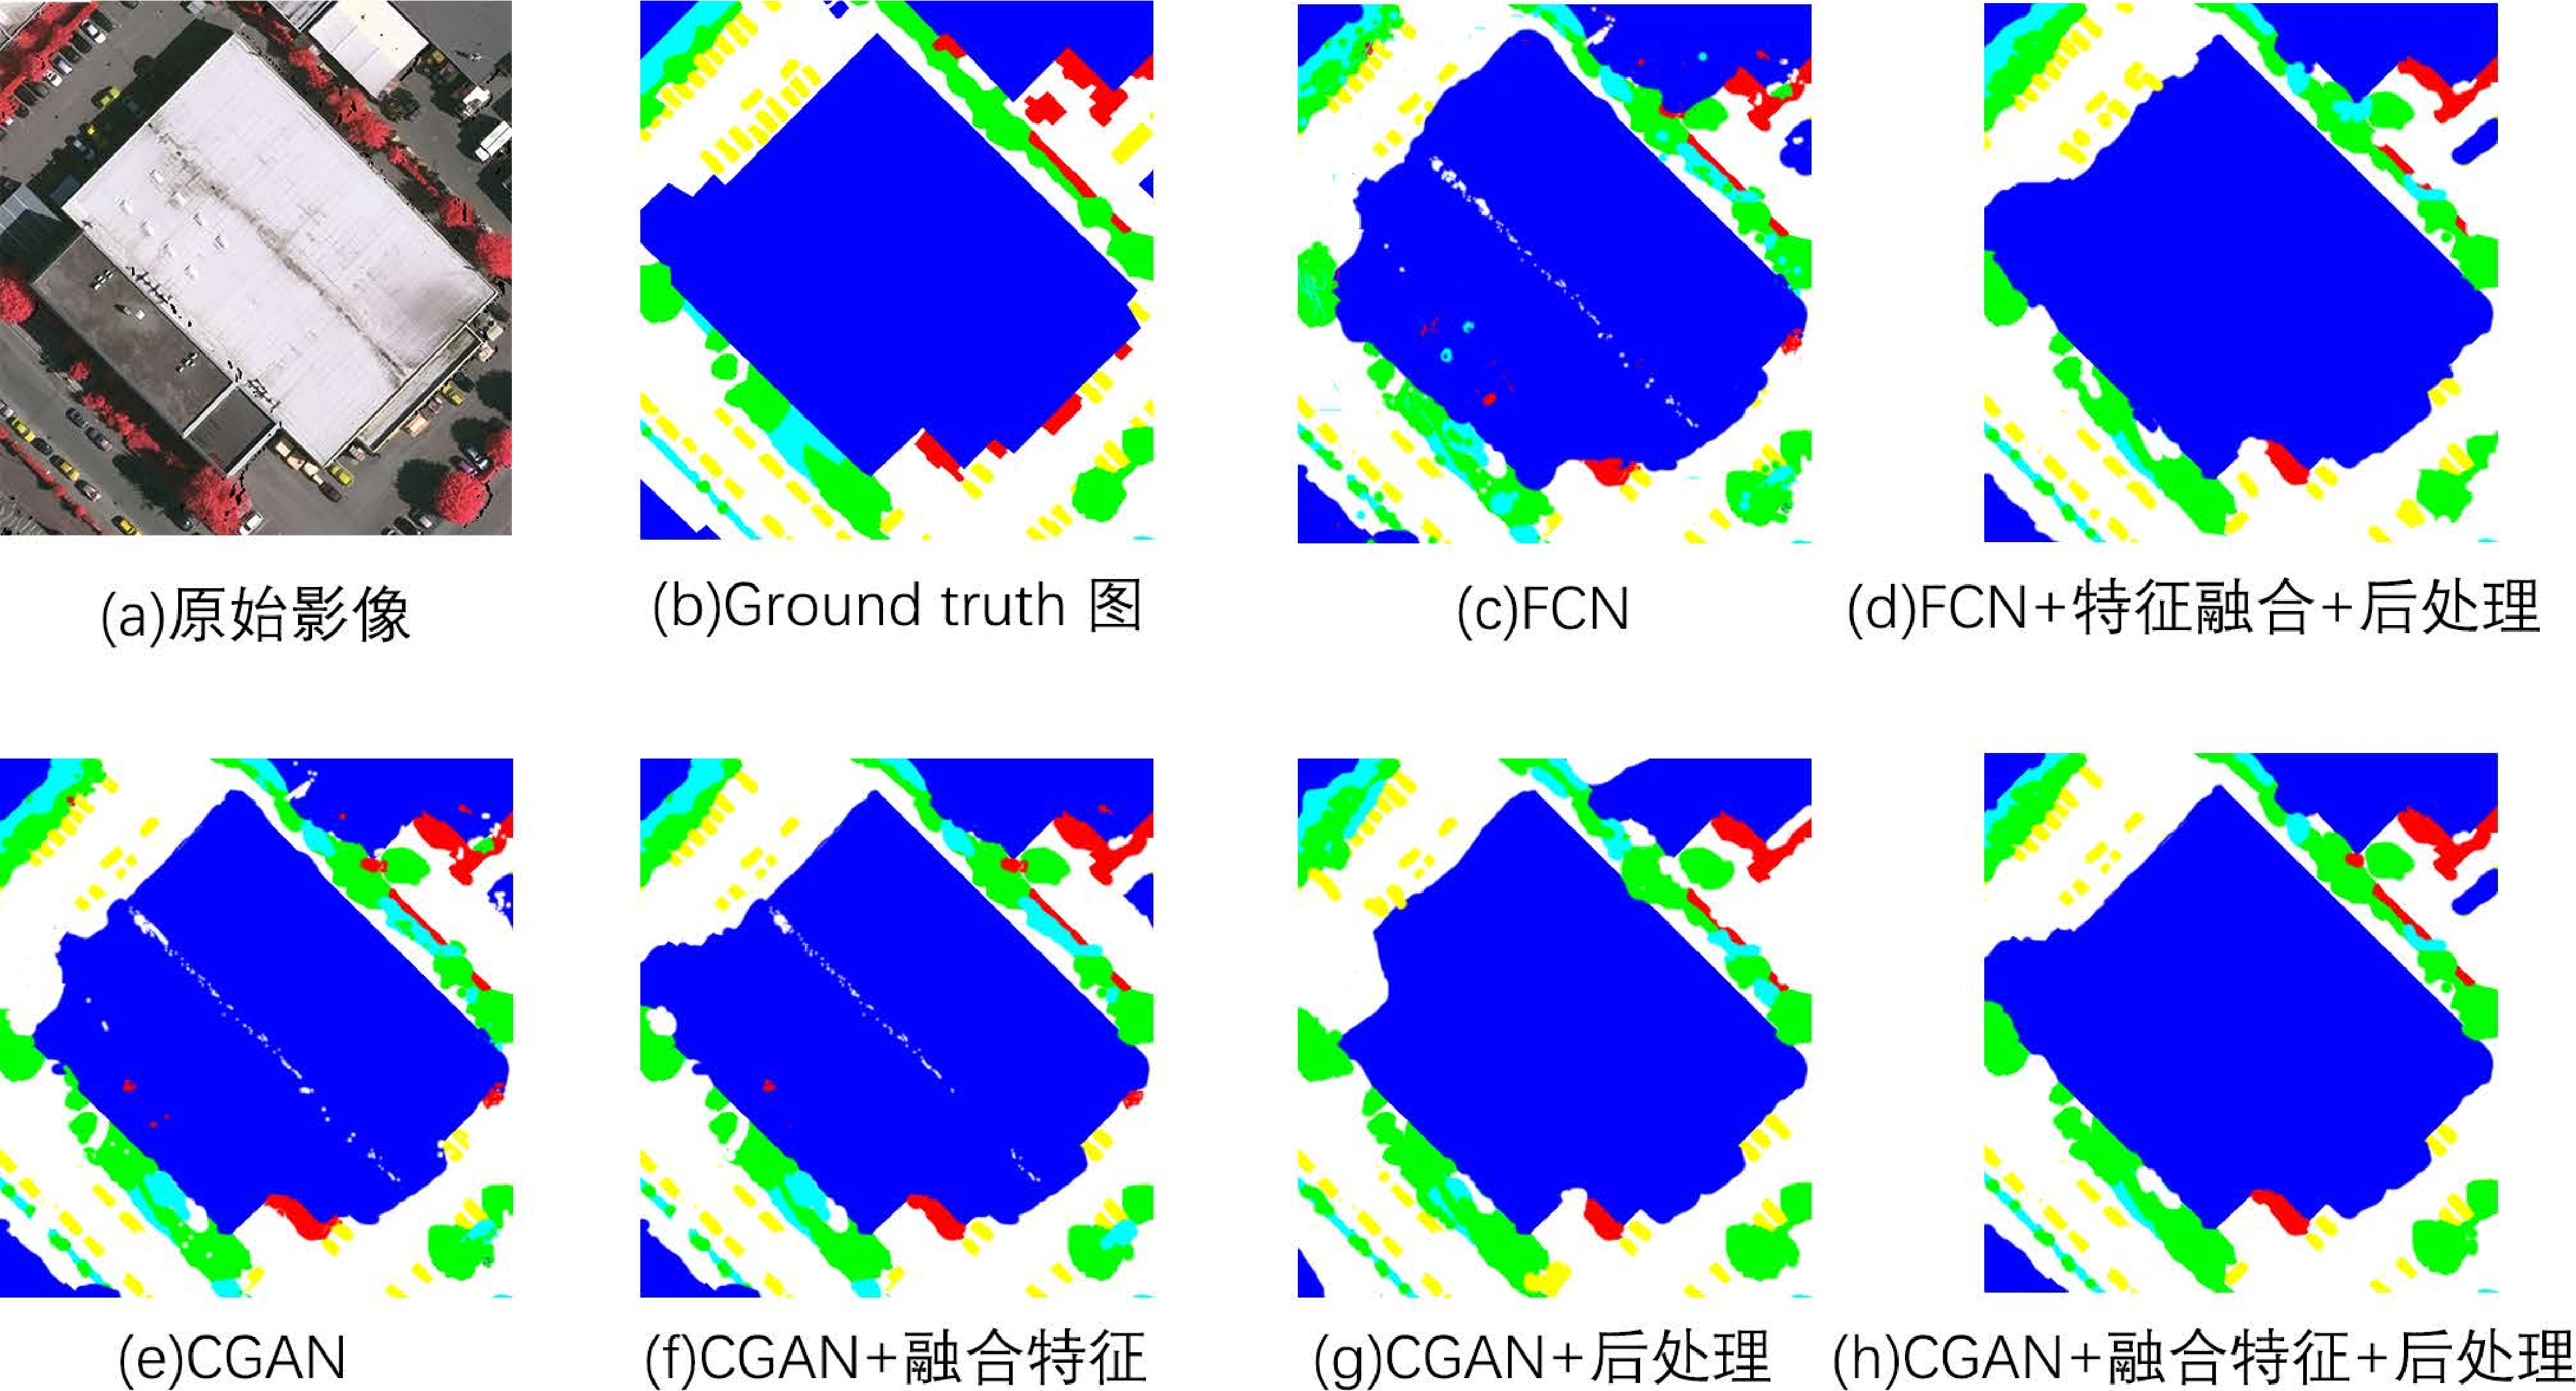
\includegraphics[width=1.0\textwidth]{figures/youhua_res}
    \caption{改进方法分类结果可视化图 }\label{fig:youhua_res}
\end{figure}

图\ref{fig:youhua_res} 中的(e)和(d)图比较了基于CGAN 影像分类方法和融合边界特征的CGAN 影像分类方法的分类效果,参照原始影像和真实分类Ground truth 图,可以看到融合了边界特征的影像分类方法在处理图中白色建筑物与阴影区域的边界上能够得到比没有融合特征的分类方法更好的边界信息。阴影和房屋的分界线更加完整、清晰。实验结果验证了融合特征的分类方法确实能够获得更清晰、准确的地物分类边界,同时能提升CGAN 影像分类方法的精度。

\begin{table}[!h]
    \centering
    \caption{后处理对CGAN 影像分类的影响}\label{tab:post_cgan}
    \begin{tabular}{p{4cm}ccccccc}
        \toprule
        方法          & 地面      & 低矮植被  & 树木      & 建筑物    & 车辆      & OA        & mIoU      \\
        \midrule
        CGAN          & $83.78\%$ & $74.47\%$ & $82.40\%$ & $87.64\%$ & $78.83\%$ & $80.15\%$ & $61.83\%$ \\
        CGAN + 后处理 & $83.98\%$ & $76.92\%$ & $82.94\%$ & $87.85\%$ & $79.14\%$ & $80.97\%$ & $62.04\%$ \\
        \bottomrule
    \end{tabular}
\end{table}

为了解决高分影像中因复杂特征导致的同类别地物区域出现其他类别的细碎错分问题,在对影像各像素点类别预测时,我们考虑同质性分割单元内其他像素点的类别划分影响,提出了基于辅助信息后处理的影响分类方法,改进基于CGAN 影像分类方法的细碎区域错分问题。验证实验同样在Vaihingen 数据集上进行,各类别地物的分类精度结果如表\ref{tab:post_cgan} 所示。分析各类地物的分类精度、OA和mIoU 等指标,带有辅助信息后处理的CGAN 影像分类方法分类精度小幅提升,OA提升了$0.82\%$,后处理方法改善了一些细小区域的错分问题。

参考图\ref{fig:youhua_res}(e) 和(g) 的分类可视化结果,辅助信息后处理方法将白色建筑物中间的灰色污垢正确识别为建筑物的一部分,保持了整个建筑物区域的整体类别一致性。基准的CGAN 影像分类方法中则将其错分为“背景”类别,破坏了该区域的分类完整性。综合量化的分类精度和可视化的分类结果,我们可以论述基于辅助信息的后处理方法在对细碎区域的像素点进行类别预测时,结合了同质性分割单元内其他像素点的预测类别信息,一定程度上将这些细碎区域正确划分为正确的类别,保证了复杂区域的地物类别预测的空间一致性和完整性。

\begin{table*}[!h]
    \centering
    \caption{两种优化方法共同作用对影像分类的影响}\label{tab:youhua_cgan}
    \resizebox{\textwidth}{!}{
        \begin{threeparttable}[b]
            \begin{tabular}{lccccccc}
                \toprule
                方法                     & 地面      & 低矮植被  & 树木      & 建筑物    & 车辆      & OA             & mIoU           \\
                \midrule
                CGAN                     & $83.78\%$ & $74.47\%$ & $82.40\%$ & $87.64\%$ & $78.83\%$ & $80.15\%$      & $61.83\%$      \\
                CGAN + 融合特征 + 后处理 & $86.35\%$ & $81.56\%$ & $83.19\%$ & $88.36\%$ & $83.19\%$ & $\bm{85.32\%}$ & $\bm{68.17\%}$ \\
                FCN                      & $81.14\%$ & $63.39\%$ & $79.52\%$ & $83.96\%$ & $62.39\%$ & $78.48\%$      & $58.42\%$      \\
                FCN + 融合特征 + 后处理  & $82.57\%$ & $76.87\%$ & $81.92\%$ & $85.08\%$ & $81.33\%$ & $81.87\%$      & $62.36\%$      \\
                \bottomrule
            \end{tabular}

        \end{threeparttable}
    }
\end{table*}

前面的实验结果证明了融合边界特征和基于辅助信息后处理这两种改进方法均能提高基于CGAN 影像分类方法的分类精度,现在我们将这两种改进思路同时作用于基于CGAN 的影像分类中。同时,也将改进方法引入经典的FCN 分类模型中,比较这两种方法共同作用的分类效果。在 Vaihingen 数据集上的分类结果如表\ref{tab:youhua_cgan} 所示。分析表\ref{tab:youhua_cgan} 的分类结果,同时将融合边界特征与后处理这两种操作应用到基准的FCN 和基于CGAN 的分类模型中,均能提升影像的分类精度。其中,融合边界特征和带有后处理操作的CGAN 影像分类方法效果提升最明显,OA 精度达到$85.32\%$,mIoU 则提升到$68.17\%$,相比基准的基于CGAN 影像分类方法,分别有 $5.17\%$ 和$6.34\%$ 的绝对精度值的提升。对于FCN 模型,两种优化方法也提高了模型的分类精度。

图\ref{fig:youhua_res}(c)、(d)、(e) 和(h) 分别对应FCN 和基于CGAN 的基准方法与优化后的方法分类的可视化结果,从图中的分割结果可以发现,融合边界特征与后处理,影像地物边界的划分更合理,此外,同类别内的地物类别更加完整,减少了细碎的错分区域。

\begin{table*}[!h]
    \centering
    \caption{SVM 与RF 算法最优模型参数}\label{tab:param_svm}
    \begin{threeparttable}[b]
        \begin{tabular}{lll}
            \toprule
            方法                & 模型关键参数                                    & 值 \\
            \midrule
            \multirow{3}*{SVM } & 核函数                                  & RBF(径向基函数)\\
                                & 惩罚因子C                               & 1.2 \\
                                & 核函数参数$\gamma$                     & 0.1 \\
            \cline{1-3}
            \multirow{5}*{RF}  & 最大特征数(max\_features)              & 14 \\
                                & 树的数目(n\_estimators)                & 10 \\
                                & 最大树深度(max\_depth)                 & 11 \\
                                & 分裂需要最小样本数(min\_samples\_split) & 194 \\
                                & 叶节点最小样本数(min\_samples\_leaf)    & 85 \\

            \bottomrule
        \end{tabular}

    \end{threeparttable}
\end{table*}

为了进一步验证本文提出方法的有效性,本文基于相同的实验影像数据,与传统的遥感影像分类方法进行了对比实验。文中以支持向量机(Support Vector Machine,SVM) \cite{maulik2017remote}和随机森林(Random Forest,RF)\cite{belgiu2016random} 这两种常用的机器学习方法分类结果作为影像分类参照组。具体操作是,首先以正射三波段影像和DSM 影像组成的四波段影像作为实验数据,基于高分影像面向对象分类理论,使用SLIC 超像素分割方法处理影像得到不同的对象(分割单元);然后对分割后的对象进行特征提取,文中主要从颜色、几何、纹理三个角度提取对象特征,共计25个特征;最后,分别采用SVM 和RF 这两种机器学习方法对训练样本进行训练,并将学习到的模型对验证集影像数据进行分类验证。两种分类方法均采用网格搜索法\cite{han2012parameter}寻找最优模型参数,模型的最优实验参数如表\ref{tab:param_svm} 所示。


表\ref{tab:compare_traditional} 所示为SVM、RF 两种机器学习方法和FCN 分类方法以及本文提出的融合边界特征与辅助信息后处理的CGAN分类方法的分类精度比较结果。从表中分类精度结果可知,本文提出的分类方法对各类地物的分类效果最佳,融合边界特征和后处理的FCN 方法分类精度次之,传统机器学习分类方法的精度相对较差,且RF 的分类精度略好于SVM 分类方法。从OA 精度和mIOU 指标进行分析,本文提出的基于CGAN 最优的分类方法精度相比融合边界特征和后处理的FCN 方法,基准FCN 分类方法,RF 和SVM 分类方法,OA 精度分别提升了$3.45\%$、$6.84\%$、$10.40\%$ 和$12.04\%$;mIoU 值则分别提升$5.81\%$、$9.75\%$、$13.80\%$ 和$14.23\%$。文中与高分影像传统分类方法和深度学习领域的分类方法的对比实验结果验证了本文提出的方法的有效性。

\begin{table*}[!h]
    \centering
    \caption{本文方法与其他方法分类精度比较}\label{tab:compare_traditional}
    \resizebox{\textwidth}{!}{
        \begin{threeparttable}[b]
            \begin{tabular}{lccccccc}
                \toprule
                方法                     & 地面      & 低矮植被  & 树木      & 建筑物    & 车辆      & OA             & mIoU           \\
                \midrule
                SVM                      & $77.95\%$ & $59.12\%$ & $75.40\%$ & $81.39\%$ & $74.59\%$ & $73.28\%$      & $53.94\%$      \\
                RF                       & $78.20\%$ & $59.47\%$ & $77.64\%$ & $81.88\%$ & $71.96\%$ & $74.92\%$      & $54.37\%$      \\
                FCN                      & $81.14\%$ & $63.39\%$ & $79.52\%$ & $83.96\%$ & $62.39\%$ & $78.48\%$      & $58.42\%$      \\
                FCN + 融合特征 + 后处理  & $82.57\%$ & $76.87\%$ & $81.92\%$ & $85.08\%$ & $81.33\%$ & $81.87\%$      & $62.36\%$      \\
                CGAN + 融合特征 + 后处理 & $86.35\%$ & $81.56\%$ & $83.19\%$ & $88.36\%$ & $83.19\%$ & $\bm{85.32\%}$ & $\bm{68.17\%}$ \\
                \bottomrule
            \end{tabular}

        \end{threeparttable}
    }
\end{table*}

综上所述,本章提出的融合边界特征的改进和基于辅助信息后处理的改进方法均提升了基于CGAN 影像分类方法的分类效果,且分类效果优于传统机器学习分类方法。Vaihingen 数据集上量化精度和目视评估结果均验证了这两种优化方法的正确性。


\section{本章小结}
\label{sec::chap04-6}
本章针对高分影像分类结果中存在边界混淆、同类地物存在细碎错分区域的问题,分别从增强分割模块中高阶特征图的边界位置特征信息和像素点分类后处理这两个角度改进基于CGAN 影像分类方法的不足。首先使用TFSV-IT2FCM 聚类分割方法对高分影像预处理,获取影像的同质性分割单元。然后,将影像的边界特征信息融合到反卷积上采样的特征图中,提升高阶语义特征的边界位置信息表达能力,提出了融合边界特征的 CGAN 影像分类方法,用于解决影像混淆的分类边界问题。接着,对模型像素点预测的类别分布概率进行加权优化,考虑同质性分割单元内其他像素点的类别预测概率,优化该像素点的概率预测结果,提出基于辅助信息后处理的CGAN 影像分类方法,由于提升同类地物分类结果的空间一致性。最后,分别在Vaihingen 数据集上进行实验验证。量化和目视的实验结果均证明了这两种优化方法的正确性和可行性。
